\documentclass[11pt]{article}
\usepackage{amsmath}
\usepackage{amssymb}
\usepackage{geometry}
\usepackage{graphicx}
\usepackage{placeins}
\usepackage{multirow}
\usepackage{float}
\usepackage{amsmath}
\usepackage[normalem]{ulem}
\usepackage[table,xcdraw]{xcolor}
\usepackage{datetime}
\settimeformat{hhmmsstime}

\graphicspath{{figures/}}

\setlength{\parskip}{\baselineskip}%
\setlength{\parindent}{0pt}%
\geometry{left=2.5cm,right=2.5cm,top=2.5cm,bottom=2.5cm}

\title{The Economics of Cybersecurity --- Lecture 11 Notes}
\date{April 2, 2024}

\author{Adam Hastings}


\begin{document}
\maketitle

\section{Introduction}

We are going to touch on Mechanism Design, cover some of the well-known and celebrated results from this field, and then discuss how we can apply mechanism design to problems facing security.

\section{Game Theory Recap}

\subsection{Backwards Induction}

% Cake cutting example?


\section{Control Systems}

What does this look like? (A system diagram! Remember HW1?)

\section{Mechanism Design}

\subsection{The Divide-and-Choose Mechanism}

\begin{itemize}
    \item The paper begins with a description of the divide-and-choose mechanism. Can someone tell me what this is? (A mechanism for creating a fair split )
    \item We learned game theory last week. Let's write this out as a game:
    \begin{itemize}
        \item Players: $\mathcal{I} = \{1,2\}$
        \item Actions: 
    \end{itemize}
    \item Does this work for more than two players? What if we wanted to split a cake three ways?
    \begin{itemize}
        \item I could cut a cake into three pieces. What does this look like as a game?
        \begin{itemize}
            \item Players: $\mathcal{I} = \{1,2,3\}$
            \item Actions: $\mathcal{A} = \{a_1 = \text{Choose piece 1}, a_2 = {Choose piece 2}, a_3 = {Choose piece 3}$
            \item Utility: $u_i = \text{size}(a)$
        \end{itemize}
    \end{itemize}
\end{itemize}

\subsection{Auctions}

{\it Note: Much of this section on auctions is inspired by and borrowed from Tim Roughgarden's class notes on Algorithmic Mechanism Design---a class here at Columbia! Go take it if this topic interests you.}

Auctions are a classic area of study in mechanism design.
Auctions are one of those things that may seem so simple you don't need to study them at all, but it turns out that there are many different types of auctions and many reasons why you might choose form over another.

We're going to go over auctions first to help us develop a taste for what mechanism design and what its uses are before we try to tackle the mathematical definition of it. 

\subsection{Simple Auctions (English auctions or open outcry auctions)}

Let's start with an open-air auction at, say, and art gallery:
\begin{itemize}
    \item Bidders will place bids that are monotonically increasing. There is usually minimum ``bid increment'' of about 10\%, so that if the previous bid is \$100, you have to bid at least \$110, not \$100.01. 
    \item The bidding repeats until a highest bid is placed. The person who places the highest bid pays the value of the bid and receives the item.
\end{itemize}

{\it From a computability perspective: What is the complexity of this algorithm?} It is $O(n)$, where $n$ is the number of bids\footnote{Technically $O(n)$ transactions, but then computing the maximum bid is $O(1)$}. If you're in an auction house, maybe that is tolerable, but what if you're in a situation where time is critical? 

{\it Ask: Does anyone know of any real-world situations where the runtime of an auction is of critical importance?}
Online advertisements. Ad personalization is a huge part of the online economy, and pays for a large portion of the tech economy. But did anyone know that it's all based on auctions? Google or Facebook provide your data (age, sex, search history, etc.) and then advertisers place bids based on your data to determine which advertisement you see. This all happens on the order of milliseconds. This can't rely on a $O(n)$ process if you consider the relative slowness of network connections. It relies on a $O(1)$ auction\footnote{Technically you still have to find the highest bid, which is $O(n)$. But the number of sequential transactions between auction players and auction house is now $O(1)$}.

{\it What are some of the other drawbacks of this auction design?} It is very public. Even if the auction is done anonymously, you are revealing to the market what your valuation of goods is; if the same good or type of good (like ads) is auctioned repeatedly, this public information can be used against you. 

{\it Ask: If you're an auction designer, how can you design an auction that doesn't require a back-and-forth $O(n)$ algorithm? And perhaps one that isn't quite so public?} (Answer: Students will probably suggest a first-price sealed auction, a.k.a. a ``silent auction'')


\subsection{First-price sealed bids}

This is another type of auction commonly seen in fundraising events: People interested in the good write their bids on a piece of paper, seal it in an envelope, and drop it in a basket; the person who writes the highest bid pays the amount on the bid and receives the good.

What are the available strategies? 
\begin{enumerate}
    \item You can bid the amount of how much you value the auctioned good. E.g. if you value the good at \$100, you could place your bid at \$100. {\it Is this a rational strategy?}
    \begin{itemize}
        \item No. If your valuation is \$100, then you are indifferent between having \$100 or having the good. If you were to win the auction with this bid, your net utility would remained unchanged.
    \end{itemize}
    \item You can (and should) bid less than your valuation of the good. {\it Ask: what's the challenge here?}
    \begin{itemize}
        \item It's difficult to compute how much less than your valuation you should bid, because this relies on knowing information about the valuations of all the bidders you're bidding against. You're forced to do a Bayesian analysis of the game and---based on your estimates of the other players---you ideal strategy is to bid the smallest amount possible that you think will still win you the auction.
        \item An extension of this is that it's likely that, in the end, the auctioned good goes to a bidder whose valuation was {\it not} the highest out of the bidders, if they happened to do their calculations differently. This is an economic inefficiency! In an ideal auction, the good would go to the person who has the highest valuation of the good.
    \end{itemize}
\end{enumerate}

\subsection{Vickrey auctions and Generalized Second Price auctions}

In terms of game theory an mechanism design, you are forced to engage in strategic bidding. {\it Ask: Imagine you are auction holder, like Google or Ebay or Sotheby's. Does anyone know of an auction ``game'' you can design that eliminates the problem of strategic bidding?}

A commonly-used auction design---one that has been used for centuries---is the {\it sealed-bid second price auction}, also known as the {\it Vickrey auction}\footnote{named after William Vickrey, professor of economics here at Columbia who was the first to describe the mathematical properties of the sealed-bid second-price auction. For this and other work on incentives under asymmetric information, Vickrey was the co-recipient of the 1996 Nobel Memorial Prize in Economics. Fun fact---William Vickrey is also regarded by many to be ``the father of congestion pricing'', which, if you've been following the news, is a politically hot topic as Governer Hochul has recently approved congestion pricing for New York City south of 60th st. }
In a Vickrey auction, everyone submits one bid ($O(1)$ transactions) the price goes to the person who submits the highest bid, but the amount they pay is the price of the {\it second-highest bid}.

{\it How does this change the stragies of the players?} I'm not going to go through the proof---but there is a proof---that this auction design has a dominant strategy ({\it Someone remind me---what's a dominant strategy?} One that is optimal regardless of all the other players' actions). And the dominant strategy, believe it or not, is to simply bid your true valuation! 

The benefits over the sealed-bid first-price auction:
\begin{itemize}
    \item If you are a bidder, your strategy is very simple! Just bid your true valuation. You don't need to estimate other player's strategies or valuations
    \item It is incentive compatible. In fact, because there is a dominant strategy, this ``game'' has a special name in game theory: It is a {\bf dominant strategy incentive compatible game}, or {\bf DSIC} game. 
    \item The auctioned good always goes to the bidder with the highest valuation.
    \item If you're the highest bidder, you certainly walk away happy---you end up paying less than your valuation! You end up with positive surplus utility. 
    \item Computationally efficient (1 transaction from each bidder, finding two highest bids is $O(n)$).
    \item Privacy-preserving (same with first-price sealed bid auction).
\end{itemize}

This is not just academic hot air---these are used in the real world:
\begin{itemize}
    \item Facebook used a Vickrey-Clarke-Groves auction, which is a generalization of the Vickrey auction that extends an auction of one good into an auction of multiple goods.  
    \item Google used a Generalized Second Price auction (similar to a Vickrey auction with a few modifications)
    \item I read somewhere that due to ``trust issues'' among advertisers there has been a switch to different types of auctions (source: https://www.cmu.edu/tepper/news/stories/2020/april/display-advertisting-research-ravi.html) but I haven't really been able to corroborate this (I found conflicting information when I looked).
\end{itemize}

Pretty cool, right? 

Do you understand why mechanism design is called ``reverse game theory?'' The ``game'' of mechanism design is {\it designing a game} (like an auction) whose rules lead strategic players to choose actions that improve overall welfare and utility. 

{\it Any questions?}

\subsection{Mathematical Definition}

The definition of a mechanism is similar to that of a game:

\begin{itemize}
    \item A set of players $\mathcal{I}, |\mathcal{I}| = n \in \mathbb{N}$
    \item A set of outcomes $\mathcal{O} = \{o_1, o_2, o_3...o_k\}$
    \item Each agent $i \in \mathcal{I}$ has private information $\theta_i \in \Theta_i$
    \item Each agent $i$ has a utility function $u_i : \mathcal{O} \times \Theta_i \rightarrow \mathbb{R}$
    \item Utility is assumed to be of the quasi-linear form $$u_i(o, \theta_i) = v_i(o, \theta_i) - p_i(\theta_i)$$ where $v_i : \mathcal{O} \times \Theta_i \rightarrow \mathbb{R}_{\geq 0}$ represents an arbitrary valuation function and $p_i \mapsto \mathbb{R}$ 
    \begin{itemize}
        \item If $o \in \mathcal{O}$ is an outcome, then $p_i$ can be thought of as the cost (or price) imposed upon player $i$ for that particular outcome $o$. 
    \end{itemize}
    \item The social welfare $W$ can be defined as the collective summation of all agents valuations, that is \begin{equation}W(o, \theta) = \sum_{i \in \mathcal{I}} v_i(o, \theta)\end{equation}
\end{itemize}

What we've talked about previously in the class is that the state of security is often an economic failure, where we are in a socially suboptimal state because of things like misaligned incentives, prisoners dilemmas, and tragedies of the commons. 
So if you're a social planner and you want to maximize for everyone, your goals is to find the outcome $o$ that maximizes 
$$ \max_{o \in \mathcal{O}}~SW(o, \theta)$$.

{\it Question: If you're the social planner, why are you trying to find the $o$ that maximizes social welfare? Why not try to find the $\theta$ as well?} Answer: Because you can't control people's private information and can't control their internal preferences!

This leads to a somewhat obvious problem though: If we are the social planner and are trying to maximize welfare, you are relying on the players' self-reported $\theta_i$ to find the $o$ that maximizes welfare. A self-interested non-cooperative player may lie about their $\theta_i$ to try to increase their own personal welfare. 

For example, consider the naive cake cutting protocol. Player X may 

\section{Mechanism Design in Behavioral Economics}

Recall my paper ``How much is performance worth to users?'', where I measured users' willingness to accept performance losses on their personal devices. 

TODO discussion on incentive compatibility. 

\subsection{Single Discrete Binary Choice Mechanism}

\subsection{Best-Worst Scaling}

\subsection{}

\section{Workshop Report}

\subsection{Formula 1 and "dirty air"}

\begin{itemize}
    \item The workshop report mentioned something about Formula 1 racing. {\it Anyone remember the name of the ``problem''}
    \item Last class, Gabe mentioned how game theory is used in international relations, but not strictly in a mathematical or quantitative way. 
    \begin{itemize}
        \item Which is still a perfectly valid application, in my opinion. 
    \end{itemize}
    \item This workshop report is maybe an analogue of that idea but applied to mechanism design and security.
    \item As we've just seen, mechanism design can be a purely mathematical pursuit.
    \item Or we can ditch the math and just apply the themes. 
\end{itemize}

\section{Braess's Paradox}

{\it Ask: What do we think---do we need a social planner (i.e. government) to come in and solve all our problems?}

I want to point out that if you don't fully understand the system you're modifying, you can very easily make things worse. 

Imagine there are two town, separated by a mountain range. There is one highway to the north, and one highway to the south. 
Connecting the highways to the towns are smaller country roads.  
The highways take 10 minutes to drive, and the country roads take 4 minutes, so no matter on which route you take, it takes 14 minutes to drive from Town A to Town B.

Suppose 1200 cars drive from Town A to Town B every hour. 

\begin{figure}
    \centering
    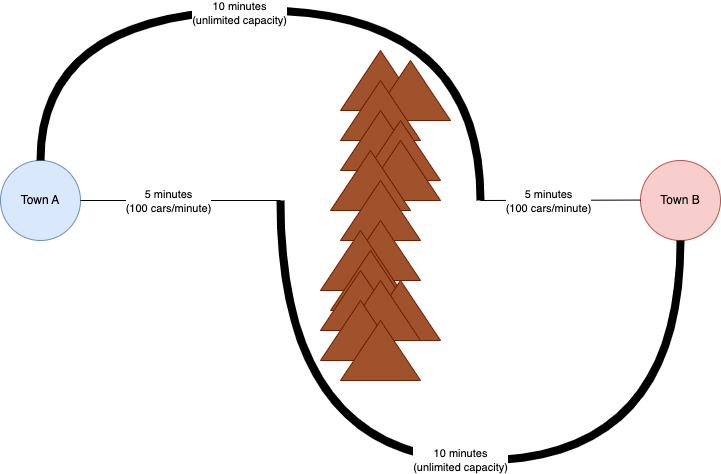
\includegraphics[width=5in]{braess_1.png}
    \caption{Before the tunnel, it takes 1200 cars 14 minutes to travel from Town A to Town B}
\end{figure}

% An urban planner looks at this and says, {\it why don't we build a tunnel through the mountains, connecting the country roads? It will take 2 minutes to drive through the tunnel, therefore we'll shorten the drive from 15 minutes to 12!}

Let's look at this as a game from the persepctive of the players. 

\begin{itemize}
    \item {\it What is the number of players?} $\mathcal{I} = \{1,2,\ldots 1200\}$.
    \item {\it What is the set of actions available to the players?} Take the north route or take the south route: $a = \{\text{North}, \text{South}\}$.
    \item {\it How much utility do players get from either strategy?} In both cases the players are trying to minimize negative utility (lost travel time). We can write this as $u(R_N) = u(R_S) = -14{:}00$.
    \begin{itemize}
        \item {\it Why is the utility negative?} Negative utility represents a bad thing. In this case, the bad thing is travel time. So the longer the drive time is, the greater the negative utility is, and the worse it is.
    \end{itemize}
\end{itemize}


{\it So what is the strategy?} The strategy is to maximize utility, i.e. choose $\operatorname*{argmax}_a (u(a))$.

Since the utility of both is equal, we can assume that 50\% of players will choose the north route and that 50\% of players take the south route. In terms of game theory, we call this a {\it mixed strategy} since strategies are probabilistic in nature. Just in case you end up reading or working more on game theory later on and you see the term {\it mixed strategy}, that's all it means.


{\it Let's say you're an urban planner, and you just been hired by the Inter-Town Transit Authority to reduce the travel time between the two towns. What might you do to reduce travel times?} You could dig a tunnel through the mountains.

\begin{figure}
    \centering
    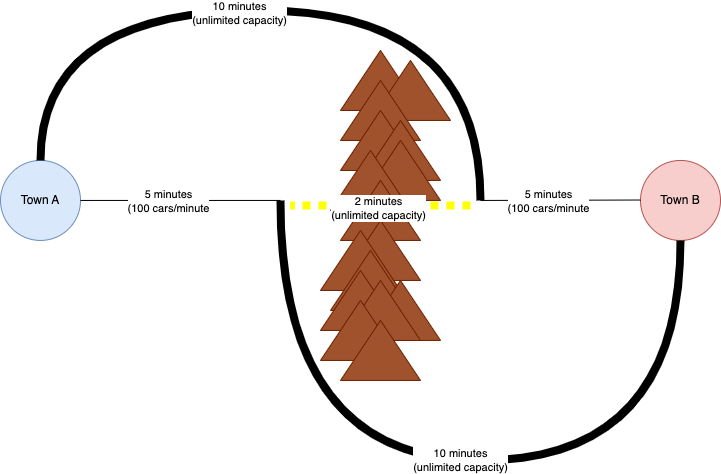
\includegraphics[width=5in]{braess_2.png}
    \caption{A naive urban planner might expect the tunnel to reduce the drive time to 10 minutes}
\end{figure}

{\it Does anyone see a problem here?} (If a student notices: We're going to incentivize all the traffic to go on the small country roads)

Let's suppose that you, the urban planner, did a little bit more research on the roads before digging the tunnel, and you found that the country roads have a limited capacity. Suppose they can only allow 12 cars/minute. 

Recall that there are 1200 cars per hour. Since there are two routes, and they're identical, we can assume that every hour 600 cars take the north route and 600 cars take the south route per hour, or 10 cars per minute. 

$$ \frac{600~\text{cars}}{\text{hour}} = \frac{10~\text{cars}}{\text{minute}}$$

Can our country roads handle this capacity? Yes. 
In other words, the travel time is unconstrained by the number of cars.
We can write the travel time of the country roads as

$$ t = \max(4, 4n/12)$$
where $n$ is the number of cars per minute.

TODO draw graph and explain!!

{\it Any questions?}

What happens if {\it every} car takes the tunnel? I.e. instead of 10 cars per minute, the country roads now have 20 cars per minute? The travel time for each stretch of the country road becomes

$$ t = \max(4, 4(20)/12) = 6{:}40~\text{minutes}$$ 

What happens if we dig the tunnel? In the best case the travel time will be 10 minutes, if there were no other cars on the road. But if everybody takes the tunnel, the travel time will be $6{:}40 + 6{:}40  + 2{:}00 = 15{:}20~\text{minutes}$. This isn't any faster than the old route, which was 14 minutes.

But what is the time of the old route now? $6{:}40 + 10{:}00 = 16{:}40$. Taking the highway is still the slowest option, but it too is slower than before!

Let's look at the game.

\begin{itemize}
    \item $\mathcal{I} = \{1,2,\ldots 1200\}$
    \item $a = \{\text{North},\text{South},\text{Tunnel}\}$
    \item $u(R_N) = -16{:}40,~~u(R_S) = -16{:}40,~~u(R_T) = -15{:}20$
\end{itemize}

Recall that the strategy is to maximize utility. The highest utility is achieved by taking the tunnel.
But note that this is no longer a mixed strategy. This is a dominant strategy! Every player is going to take the tunnel.

{\it Can someone tell me the plain-English interpretation of what I just said?} We built a tunnel. The tunnel incentivized everybody to take the tunnel. But because of the road capacity issues, this route ended up being slower than the old routes around the mountains. But the tragedy is that the old routes now also became slower as well! You can't get from Town A to Town B in 14 minutes anymore.  


\begin{figure}
    \centering
    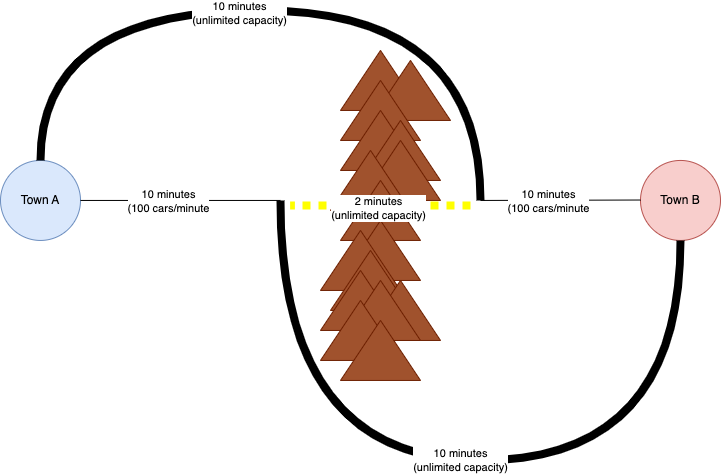
\includegraphics[width=5in]{braess_3.png}
    \caption{A naive urban planner might expect the tunnel to reduce the drive time to 12 minutess}
\end{figure}

Note that the old roads still exist! Everyone could cooperate and have 50\% take the north road and 50\% take the south road. But that's really hard to enforce! 
Because then what happens? 
That tunnel is still there, and is just too tempting---If you're the only one taking the tunnel, your travel time is 10 minutes! 

\subsubsection{Price of Anarchy}

In economics, game theory, and mechanism design, there is a concept called the {\it POA}, or {\it Price of Anarchy}.
This is a quantitative measure of the overhead imposed by agents choosing selfish behavior, and is defined as the ratio between the Nash equilibrium outcomem and the socially optimal outcome. 
In this game, the socially optimal outcome was -14 minutes while the equilibrium outcome was -15 minutes 20 seconds. 
{\it (Note that the socially optimal outcome was -14 minutes even after the tunnel is built)}.
So we have
$$ PoA = \frac{15{:}20}{14{:}00} \approx 1.095 = 9.5\%$$

In other words, the system is 9.5\% worse off because the rules of the game allow for selfish behavior which comes at the expense of the other drivers. 


In the prisoner's dilemma, we had a (-1,-1) payoff for (cooperate, cooperate) and a (-2,-2) payoff for (defect, defect). The social cost of (cooperate, cooperate) is 2 and the social cost of (defect, defect) is 4. This is a $4/2 = 2\text{X} = 100\%$ price of anarchy. {\it Any questions?}

{\it Ask: In the prisoner's dilemma, who is the social planner?} The party who has a degree of influence or control over the players, so in this case, the mob :) 

As a fun fact, the term {\it Price of Anarchy} comes from a 1999 paper ``Worst-case equilibria'' by  Elias Koutsoupias and our very own Christos Papadimitriou (although the concept of measuring the inefficiency of selfish behaviour predates this paper by quite a bit. But within the algorithmic game theory and algorithmic mechanism design, this is a very commonly-used term.)

\subsection{Extending Braess' Paradox to Security}

The general concept of what is going on here is called Braess' Paradox. 
You may have also seen this with two springs and a weight. {\it(Has anyone seen this before?)} It's a physical analog to this situtation with roads and tunnels. 
It's counterintuitive but cutting the middle string causes the weight to {\it rise}, not fall. 
The reason is because with the middle string, the two springs are acting in series, and both springs are bearing the full weight, whereas once the middle string is cut, the two springs are acting in parallel, meaning that they each are only holding half the weight. 

In traffic engineering and urban planning, it's often explained in terms of roads between two cities.



\subsubsection{Discussion}

What are the takeaways?

\begin{itemize}
    \item If we're going to meddle with systems, we have to be very confident that we fully understand the system we are meddling with. Otherwise we can make things much worse. I suppose this is a mathematical example of a perverse incentive. 
    \item {\it Any others}?
    \item The takeaway that I've led you to thus far is that a misguided planner can make things worse. Equivalently, a smart planner can make things better by doing counterintuitive roads. Imagine that you're the city planner hired to improve travel times between Town A and Town B, {\it and the tunnel already existed}. How do you think the public would react if your solution is to {\it close the tunnel}?
    \begin{itemize}
        \item Sometimes you need the political will and determination to do things that are beneficial but unpopular.
        \item {\it In general though, how do you know if you're the smart planner who is going to make things better, or the naive planner who is going to make things worse??} I don't know. Would love some answers to this question! 
    \end{itemize}
\end{itemize}


\section{Mechanism Design for Hardware Security}

This is not a peer-reviewed paper. This is a report from a workshop event a couple of summers ago, where me, Prof. Sethumadhavan, and about 50 other people from academia, industry, and government got together and discussed what mechanism design means for hardware security. 

Aside: For anyone who doesn't know, {\it Hardware Security} is exactly what it sounds like: It's a sub-field of security that focuses on securing systems from the ground up, starting from the circuit level to the physical device level and typically including up to computer architecture. 
If this is a topic that interests you, and you are not graduating this semester, there is a hardware security class in this department, taught by Prof. Sethumadhavan. 
(Today's class is really just an advertisement for other graduate-level classes at Columbia, isn't it?)

The workshop was from people who work in the hardware security area. I.e. topics like side channel detection and exploitation, hardware trojans, speculation safety, Rowhammer, hardware-based defenses like CFI, secure embedded systems, tamper-proof hardware, hardware enclaves and trusted execution environments ({\it to Simha: any others I'm missing?})
To prevent an echo chamber, there were also some people from economics and a few people who worked in government policy (next week's topic).

{\it Ask: Why did I have you read a workshop report rather than a peer-reviewed paper on mechanism design for security?} Mostly because there is no work on this topic! This is an emerging research area. The purpose of this workshop is to spur research in this direction. But mechanism design is such an interesting tool and one that security practitioners ought to have in their toolbox. It's economics applied directly to improving security. Extremely relevant to this class, (hopefully) extremely important to the field of security moving forward.

\subsection{Recommendations}

The format of the event was a mix of presentations and discussion, with the end goal of coming up with a set of recommendations for what the hardware and computing communities can do to improve hardware security through mechanism design. 

These were the recommendations we came up with {\it (write on board)}:

\subsubsection{Foster Diverse Educational, Professional, and Industrial Communities in Hardware Security}

\subsubsection{Lay the Scientific Foundations for Work that Combines Incentives and Technology}

\subsubsection{ Make Security Accountable and Explainable}

\subsubsection{Co-Develop Emerging Technologies with the Understanding of their Hardware Security Ramifications}

\subsubsection{Prioritize the Human Impact of Hardware Security}

\subsection{Discussion}

What do we think? Did we get it right? What did we miss? What did we get wrong? {\it Write recommendations on board.}

One thing I'd like to point out is that you should not assume that just because the audience of people who contributed to this list was a bunch of established professors that their level of wisdom or insight in the topic is much better than yours. Don't think of this list as infallible, and don't think of your intuitions as invalid. Like I said, this is an emerging area, so someone who has spent all their life working in security may barely have a leg up on you (if at all!) when it comes to taking an economic perspective at security problems. 

{\it Ask Simha: In retrospect, what changes would you make to the set of recommendations?}

\subsubsection{What does this have to do with auctions, study design, etc.?}

Very little! I think there is massive potential in applying mechanism design to problems of security and security policy. 

{\it Open ended discussion: What are some areas in security where we can apply what we've learned here today to solve problems in security?}
\begin{itemize}
    \item Are there mechanisms we can use to improve patching practices?
    \item Are there mechanisms we can use to get the right people to invest in security in the right places?
    \item Can we use {\it liability} as a mechanism to balance the costs of security?
    \begin{itemize}
        \item (Remember my Doctrine of Shared Burdens?)
        \item (Seems like this is happening behind the scenes in Washington---based on statements and reports, there's clear interest in getting software vendors to take on greater liability for releasing software that is full of vulnerabilities. 
        \begin{itemize}
            \item {\it What are some of the challenges here?}
            \item Most software is a tangled web of dependencies. Who heard about the xz vulnerability over the weekend? Who should be responsible if your open source dependency leads to a vulnerability in your software? (You? The open source programmer? Someone else? Who?)
        \end{itemize}
    \end{itemize}
\end{itemize}


\section{Homework}

\end{document}
